\documentclass[crop]{standalone}
\usepackage{amssymb}
\usepackage{amsmath}
\usepackage{amsfonts}
\usepackage{color}
\usepackage{tikz}
\usetikzlibrary{math}

\begin{document}
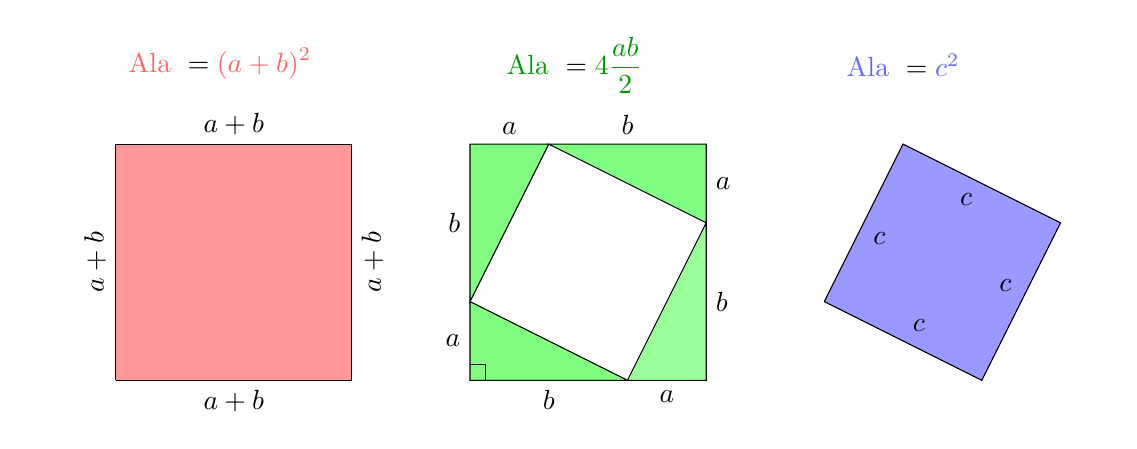
\begin{tikzpicture}

    \tikzmath{\x=4.5;}
    \tikzmath{\y=-4;}    
    \draw[fill=green!50] (\x,\y+1)--(\x,\y+0) node[pos=0.5,left]{$a$}--(\x+2,\y+0)node[pos=0.5,below] {$b$} --(\x,\y+1);
    \draw (\x,\y+0.2)-|(\x+0.2,\y+0);
    \draw[fill=green!50] (\x+1,\y+3)--(\x,\y+3)node[pos=0.5,above]{$a$}
    --(\x,\y+1)node[pos=0.5,left]{$b$}
    --(\x+1,\y+3);
    \draw[fill=green!50] (\x+3,\y+2)--(\x+3,\y+3)node[pos=0.5,right]{$a$}
    --(\x+1,\y+3)node[pos=0.5,above]{$b$}
    --(\x+3,\y+2);
    \draw[fill=green!40] (\x+2,\y+0)--(\x+3,\y+0)node[pos=0.5,below]{$a$}--(\x+3,\y+2)node[pos=0.5,right]{$b$}--(\x+2,\y+0);
    \node[rectangle,anchor=center] at (\x+1.5,\y+4) {$\begin{aligned}
        {\color{green!60!black}\text{Ala }}&={\color{green!60!black}4\frac{ab}{2}}%={\color{green!60!black}2ab}
    \end{aligned}$};
    
    \tikzmath{\x=9;}
    \tikzmath{\y=-4;}
    \draw[fill=blue!40] (\x,\y+1)--(\x+1,\y+3)node[pos=0.5,below right] {$c$}--(\x+3,\y+2)node[pos=0.5,below left] {$c$}--(\x+2,\y+0)node[pos=0.5,above left] {$c$}--(\x,\y+1)node[pos=0.5,above right] {$c$};
    \node[rectangle,anchor=center] at (\x+1,\y+4) {${\color{blue!60}\text{Ala }}={\color{blue!60}c^2}$};

    \tikzmath{\x=0;}
    \tikzmath{\y=-4;}    
    \draw[fill=red!40] (\x,\y+0)--(\x+3,\y+0) node[pos=0.5,below]{$a+b$}--(\x+3,\y+3)node[pos=0.5,below,rotate=90]{$a+b$}--(\x,\y+3)node[pos=0.5,above]{$a+b$}--(\x,\y+0)node[pos=0.5,above,rotate=90]{$a+b$};    
    \node[rectangle,anchor=center] at (\x+1.5,\y+4) {$\begin{aligned}
        {\color{red!60}\text{Ala }}&={\color{red!60}(a+b)^2}%\\
        %&={\color{red!60}a^2+2ab+b^2}
    \end{aligned}$};
    \node at (12.5,0) {};    
    \node at (-1,0) {};     
\end{tikzpicture}
\end{document}